% Document Management System Architecture
% TikZ diagram for Chapter 2

\documentclass[tikz,border=10pt]{standalone}
\usepackage{tikz}
\usetikzlibrary{shapes,arrows,positioning,fit,backgrounds}

\begin{document}

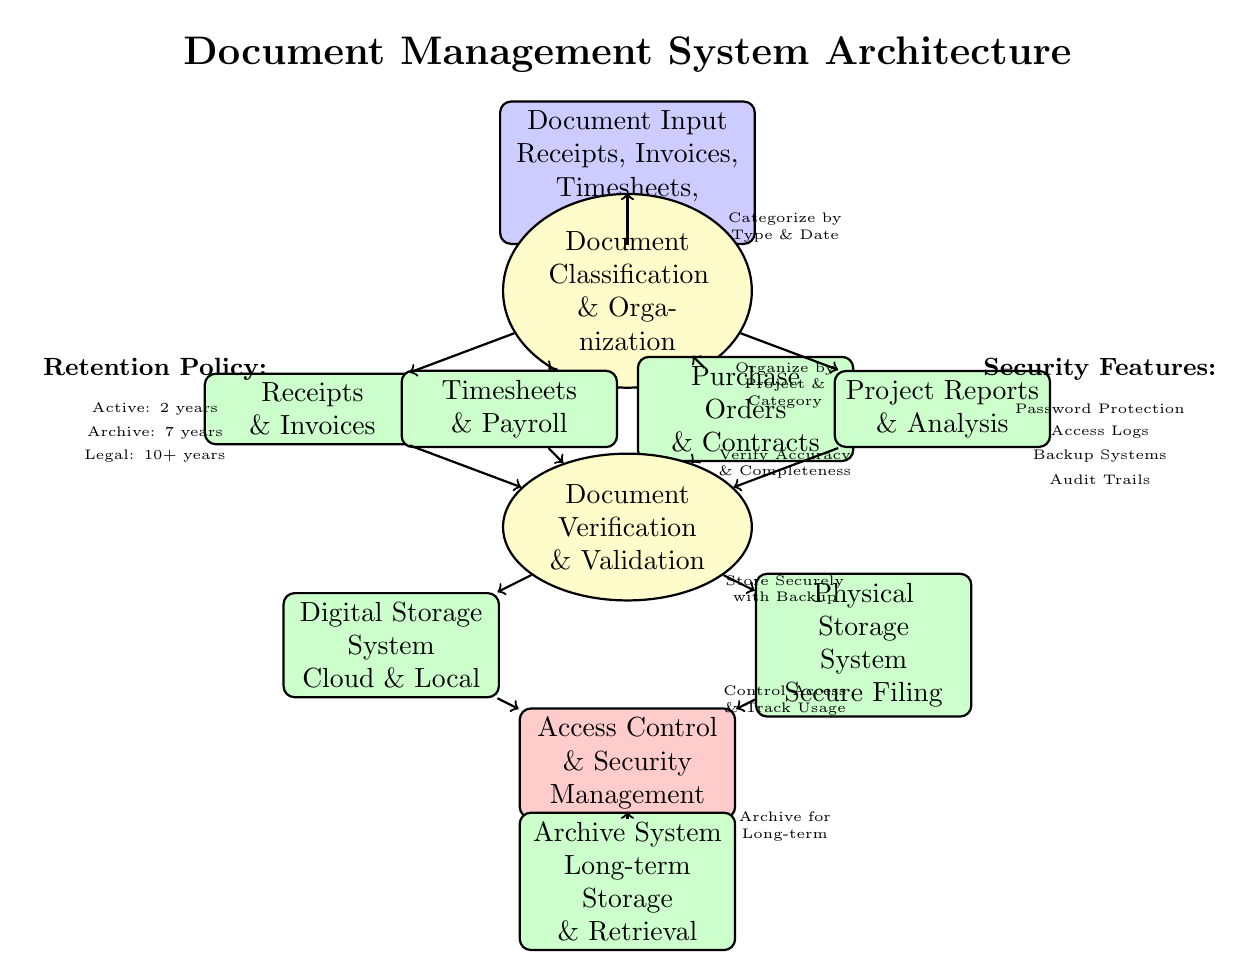
\begin{tikzpicture}[
    node distance=1.5cm,
    auto,
    thick,
    main node/.style={rectangle, draw, fill=blue!20, text width=3cm, text centered, rounded corners, minimum height=1cm},
    storage node/.style={rectangle, draw, fill=green!20, text width=2.5cm, text centered, rounded corners, minimum height=0.8cm},
    process node/.style={ellipse, draw, fill=yellow!20, text width=2cm, text centered, minimum height=0.8cm},
    security node/.style={rectangle, draw, fill=red!20, text width=2.5cm, text centered, rounded corners, minimum height=0.8cm}
]

% Title
\node[text width=12cm, text centered, font=\Large\bfseries] (title) at (0,8) {Document Management System Architecture};

% Document Input
\node[main node] (input) at (0,6.5) {Document Input\\Receipts, Invoices,\\Timesheets, Reports};

% Classification Process
\node[process node] (classification) at (0,5) {Document\\Classification\\\& Organization};

% Document Categories
\node[storage node] (receipts) at (-4,3.5) {Receipts\\\& Invoices};
\node[storage node] (timesheets) at (-1.5,3.5) {Timesheets\\\& Payroll};
\node[storage node] (purchase_orders) at (1.5,3.5) {Purchase Orders\\\& Contracts};
\node[storage node] (reports) at (4,3.5) {Project Reports\\\& Analysis};

% Verification Process
\node[process node] (verification) at (0,2) {Document\\Verification\\\& Validation};

% Storage Systems
\node[storage node] (digital_storage) at (-3,0.5) {Digital Storage\\System\\Cloud \& Local};
\node[storage node] (physical_storage) at (3,0.5) {Physical Storage\\System\\Secure Filing};

% Security Layer
\node[security node] (access_control) at (0,-1) {Access Control\\\& Security\\Management};

% Archive System
\node[storage node] (archive) at (0,-2.5) {Archive System\\Long-term Storage\\\& Retrieval};

% Arrows
\draw[->] (input) -- (classification);
\draw[->] (classification) -- (receipts);
\draw[->] (classification) -- (timesheets);
\draw[->] (classification) -- (purchase_orders);
\draw[->] (classification) -- (reports);
\draw[->] (receipts) -- (verification);
\draw[->] (timesheets) -- (verification);
\draw[->] (purchase_orders) -- (verification);
\draw[->] (reports) -- (verification);
\draw[->] (verification) -- (digital_storage);
\draw[->] (verification) -- (physical_storage);
\draw[->] (digital_storage) -- (access_control);
\draw[->] (physical_storage) -- (access_control);
\draw[->] (access_control) -- (archive);

% Process Flow Labels
\node[text width=2cm, text centered, font=\tiny] (label1) at (2,5.8) {Categorize by\\Type \& Date};
\node[text width=2cm, text centered, font=\tiny] (label2) at (2,3.8) {Organize by\\Project \& Category};
\node[text width=2cm, text centered, font=\tiny] (label3) at (2,2.8) {Verify Accuracy\\\& Completeness};
\node[text width=2cm, text centered, font=\tiny] (label4) at (2,1.2) {Store Securely\\with Backup};
\node[text width=2cm, text centered, font=\tiny] (label5) at (2,-0.2) {Control Access\\\& Track Usage};
\node[text width=2cm, text centered, font=\tiny] (label6) at (2,-1.8) {Archive for\\Long-term};

% Retention Timeline
\node[text width=3cm, text centered, font=\small\bfseries] (retention_title) at (-6,4) {Retention Policy:};
\node[text width=3cm, text centered, font=\tiny] (retention1) at (-6,3.5) {Active: 2 years};
\node[text width=3cm, text centered, font=\tiny] (retention2) at (-6,3.2) {Archive: 7 years};
\node[text width=3cm, text centered, font=\tiny] (retention3) at (-6,2.9) {Legal: 10+ years};

% Security Features
\node[text width=3cm, text centered, font=\small\bfseries] (security_title) at (6,4) {Security Features:};
\node[text width=3cm, text centered, font=\tiny] (security1) at (6,3.5) {Password Protection};
\node[text width=3cm, text centered, font=\tiny] (security2) at (6,3.2) {Access Logs};
\node[text width=3cm, text centered, font=\tiny] (security3) at (6,2.9) {Backup Systems};
\node[text width=3cm, text centered, font=\tiny] (security4) at (6,2.6) {Audit Trails};

\end{tikzpicture}

\end{document}
